\documentclass{article}
\usepackage{graphicx} % Required for inserting images
\usepackage{amsmath}
\usepackage{amssymb}
\usepackage[es]{babel}
\usepackage{hyperref}

\title{Ejercicios función cuadrática}
\author{Lorenzo Girotti }
\date{Febrero 2024}

\begin{document}
\maketitle

\section{Introducción teórica}
Con el fin de graficar las parábolas que representan a las funciones cuadráticas, vamos a introducir los conceptos de \emph{foco} y \emph{directriz} de una parábola.

\subsection{Fórmula canónica de una parábola}

Introducimos primero el concepto de expresión canónica de una parábola ya que será de vital importancia a la hora de encontrar tanto el foco como la recta directriz.

La formulación canónica de una parábola requiere de conocer su \textbf{vértice}, con coordenadas $V(h,k)$ ó $V(x_v,y_v)$ determinadas. Con ello, la fórmula queda indicada por

\begin{gather}
    \label{eq:form-canon}
    (x-h)^2=4p(y-k)\\
    (x-h)^2=-4p(y-k)
\end{gather}
Donde la ecuación (1) responde para parábolas cóncavas hacia arriba \footnote{Carita feliz} y la (2) para las que son cóncavas hacia abajo\footnote{Carita triste}; y $p$ es la distancia que separa al vértice tanto del foco como de la directriz.

\subsubsection{Pasaje a forma polinómica a canónica}

En este inciso vamos a dejar fórmulas útiles para pasar de forma polinómica a forma canónica de manera sencilla.

Forma polinómica:
\begin{equation}
    \label{eq:polinom}
    y=f(x)=ax^2+bx+c
\end{equation}

De ella, podremos conseguir las coordenadas del vértice a través de
\begin{gather}
    \label{eq:vertice}
    x_v=h=\frac{-b}{2a}\\
    y_v=k=c-\frac{b^2}{4a}
\end{gather}

 Solo restaría conocer el parámetro $p$, el cual obtenemos con

 \begin{equation}
     \label{eq:parametro}
     p=\frac{1}{4a}
 \end{equation}

De esta manera contamos con todos los ingredientes necesarios para pasar de una forma polinómica a una canónica. Veamos un ejemplo.

\paragraph{Ejemplo:} Sea $f(x)=4x^2-3x+1$, expresarla en forma canónica.

\begin{enumerate}
    \item Identificamos los coeficientes de la forma polinómica: $a=4$, $b=-3$, $c=1$.
    \item Hallamos las coordenadas del vértice:
    \begin{align*}
        x_v&=\frac{-(-3)}{2(4)}=\frac{3}{8}\\
        y_v&=1-\frac{(-3)^2}{4(4)}=1-\frac{9}{16}=\frac{7}{16}
    \end{align*}
    quedando, $V=(\frac{3}{8},\frac{7}{16})$.
    \item Calculamos el parámetro $p$, $$p=\frac{1}{4(4)}=\frac{1}{16}$$
    \item Reemplazamos en la fórmula (\ref{eq:form-canon}).
    \begin{gather*}
        (x-x_v)^2=4p(y-y_v)\\
        \left(x-\frac{3}{8}\right)^2=4\,\frac{1}{16}\,\left(y-\frac{7}{16}\right)
    \end{gather*}
\end{enumerate}

Con esta información (vértice y parámetro $p$) podemos determinar el foco y la recta directriz.

\subsection{Foco y recta directriz}
La parábola se define como la colección de puntos que \emph{equidistan}\footnote{están a la misma distancia} tanto del foco como de la recta directriz. Utilizando esto a nuestro favor, podremos encontrar tanto al foco y la recta directriz, a través del vértice y el parámetro $p$.

\paragraph{Fórmulas del foco y recta directriz:} Teniendo en cuenta que el foco se encuentra sobre el eje de simetría (es decir está por encima o por debajo del vértice), sabemos que comparte coordenada en $x$ con el vértice y dista a una distancia $p$ de la coordenada en $y$ del mismo (será hacia arriba si es cóncava hacia arriba, y hacia abajo si es cóncava hacia abajo).
\begin{equation}
    \label{eq:foco}
    F=(x_v,y_v\pm p)
\end{equation}

Para la recta directriz, sabemos que estará por debajo (corresponde el signo $(-)$) si la parábola es cóncava hacia arriba; y por arriba (corresponde $(+)$) si es cóncava hacia abajo.

\begin{equation}
    \label{eq:directriz}
    y=y_v\pm p
\end{equation}

\paragraph{Ejemplo:} Encontrar el foco y la recta directriz de la función cuadrática del ejemplo anterior.

\begin{enumerate}
    \item Hallamos el foco, teniendo en cuenta que la parábola es cóncava hacia arriba (pues $a=4>0$):
    \begin{align*}
        F&=\left(\frac{3}{8},\frac{7}{16}+\frac{1}{16}\right)\\
        &=\left(\frac{3}{8},\frac{1}{2}\right).
    \end{align*}
    \item Hallamos la recta directriz, considerando el signo negativo, puesto que debe quedar por debajo del vértice:
    \begin{align*}
        y&=\frac{7}{16}-\frac{1}{16}\\
        &=\frac{6}{16}\\
        y&=\frac{3}{8}
    \end{align*}
    \item Graficado, obtenemos la figura (\ref{fig:graf-ej}) donde podemos observar la equidistancia del punto que vive en la parábola con respecto al foco y la recta directriz.
\end{enumerate}
\begin{figure}[b!]
    \centering
    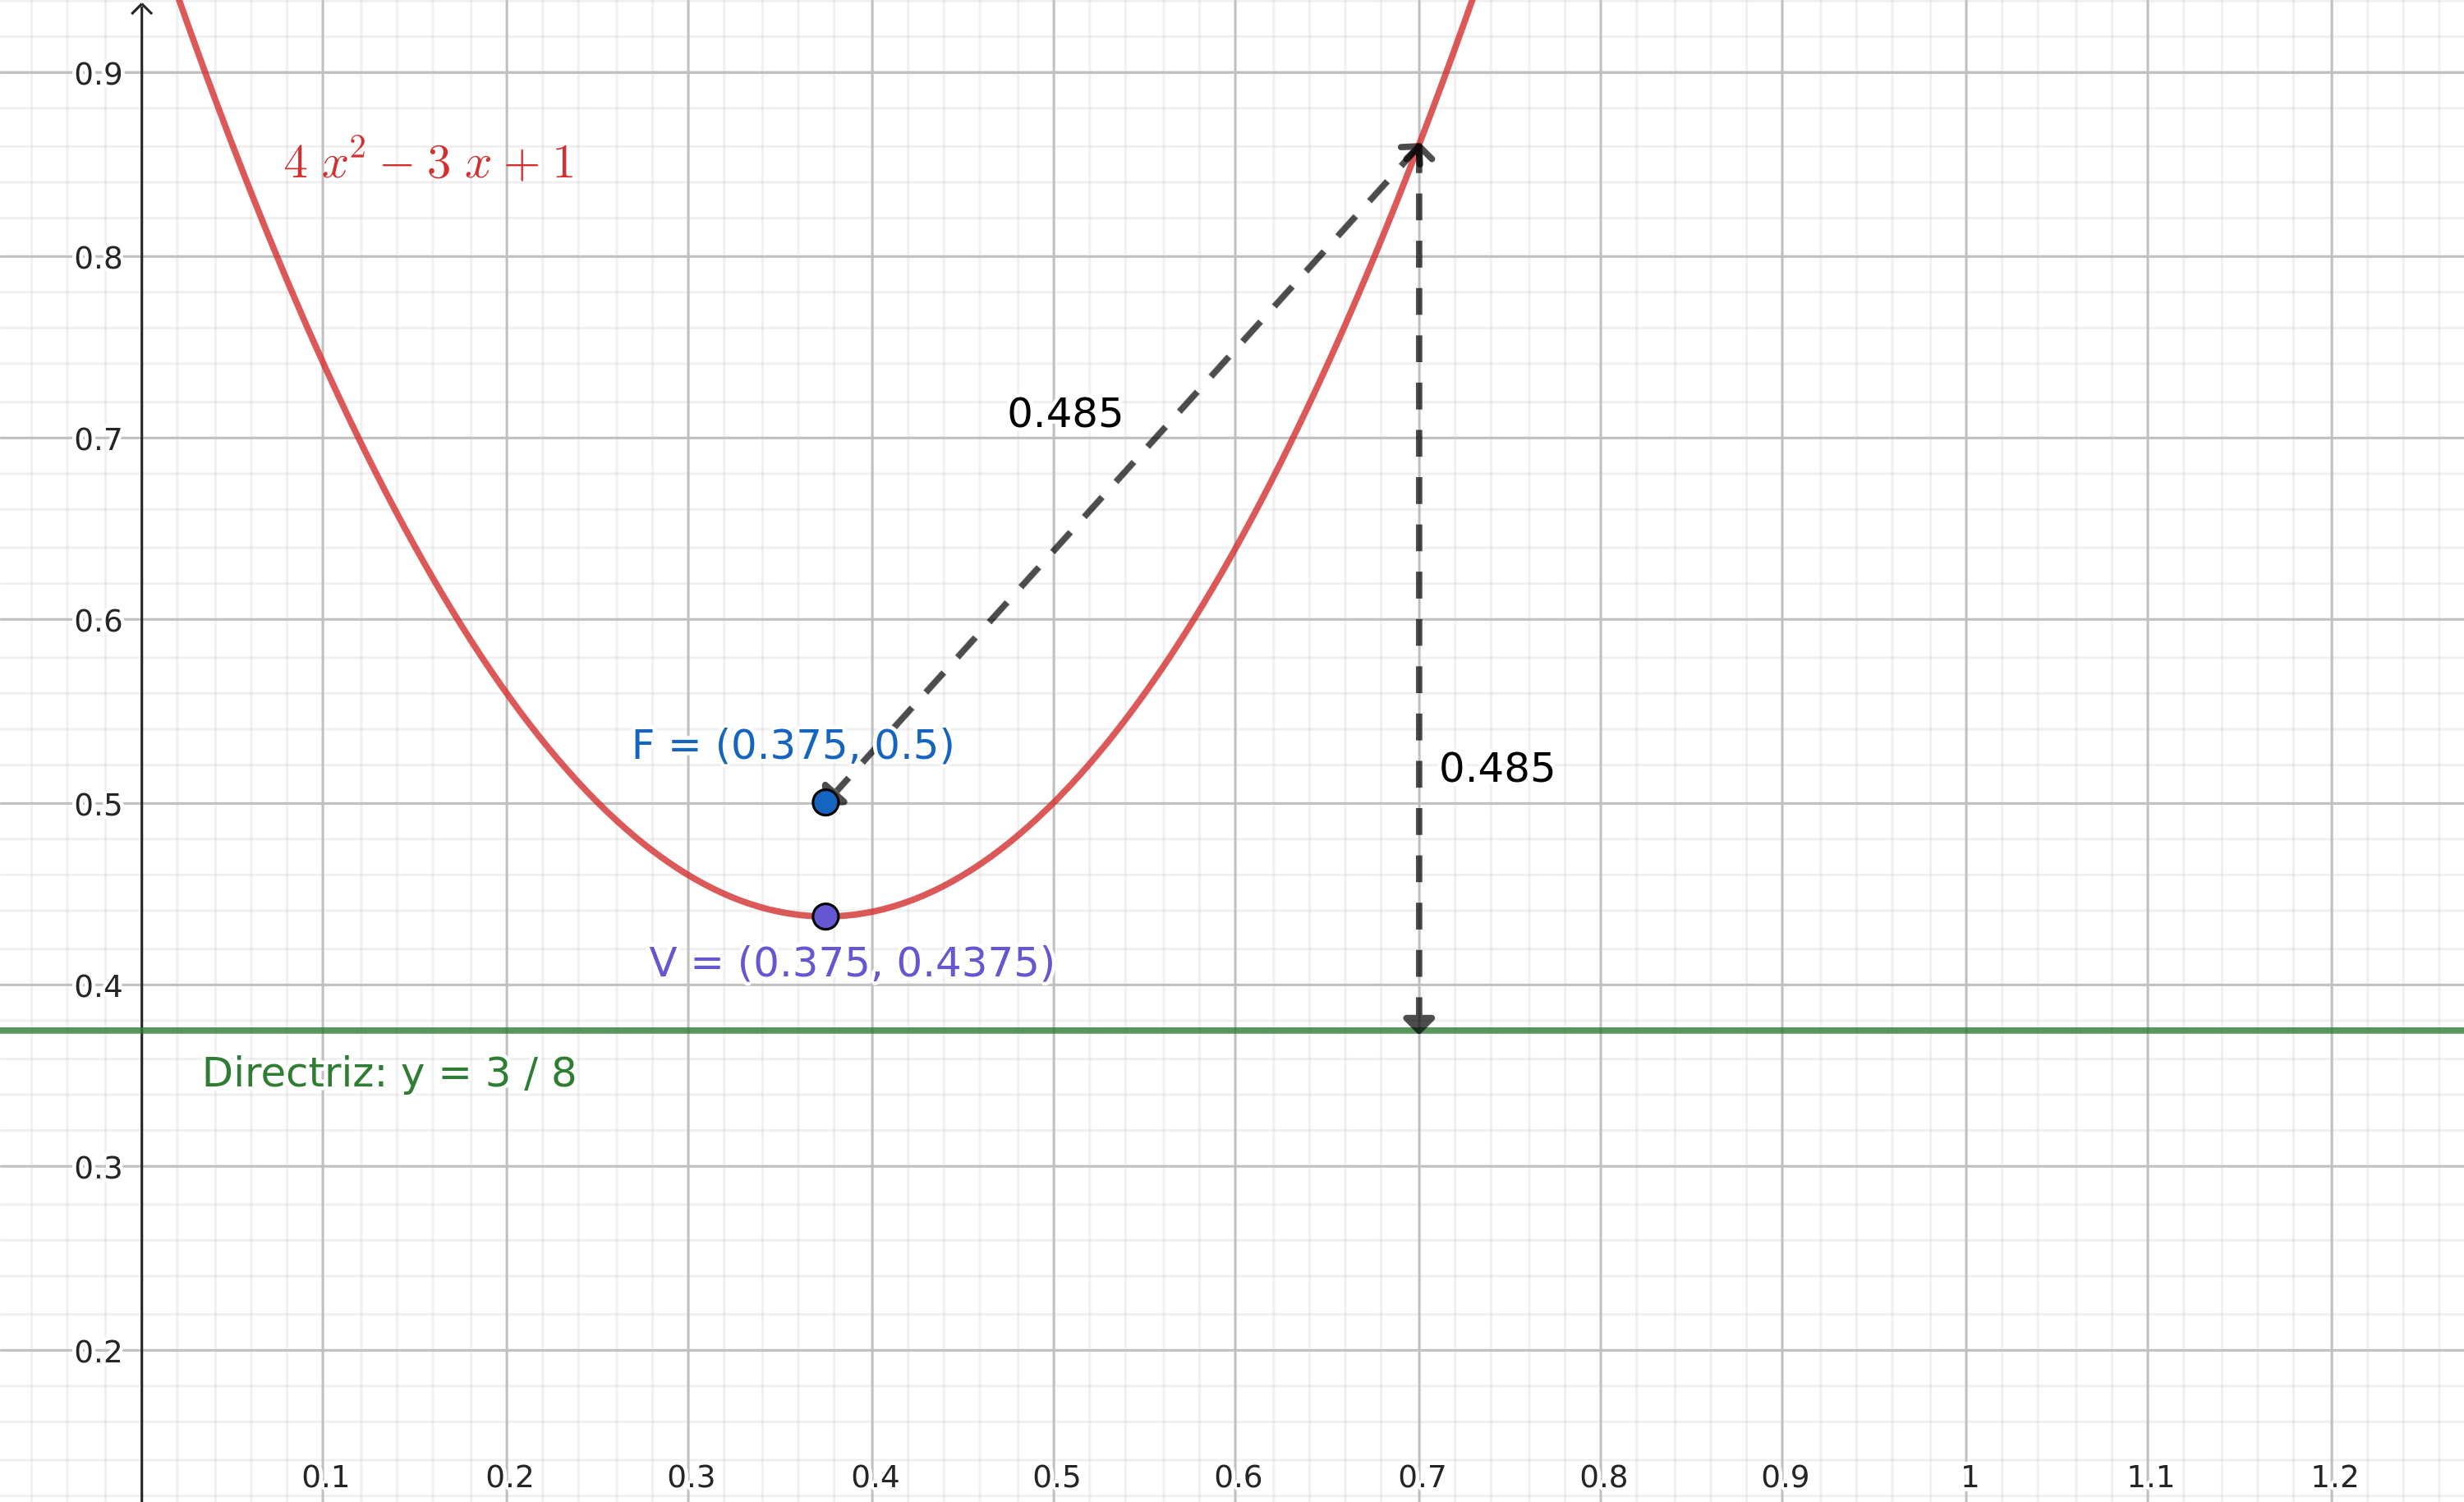
\includegraphics[width=\linewidth]{imagen.png}
    \label{fig:graf-ej}
    \caption{Gráfico de la función del ejemplo con sus elementos.}
\end{figure}

\section{Ejercitación}
Con lo aprendido, resolver los siguientes ejercicios. Justificar las respuestas.

\begin{enumerate}
    \item Hallar, de ser posible: concavidad, raíz/ces, ordenada al origen, vértice y eje de simetría de las siguientes funciones cuadráticas.
    \begin{enumerate}
        \item $f(x)=-3x^2+1$
        \item $g(x)=\frac{x^2}{4}-2x+1$
        \item $h(x)=x^2+1$
    \end{enumerate}

    \item Del inciso anterior, elegir una función y luego
    \begin{enumerate}
        \item Pasarla a su forma canónica.
        \item Hallar foco y directriz.
        \item Graficarla utilizando tabla de valores y verificar que se cumpla la equidistancia con respecto al foco y directriz en algunos puntos.
    \end{enumerate}
    
    \item Determinar si las siguientes afirmaciones son verdaderas (V) o falsas (F). Justificar.
    \begin{enumerate}
        \item Todas las funciones cuadráticas tienen exactamente dos raíces.
        \item Sólo puedo hallar raíces utilizando la fórmula resolvente.
        \item Todas las parábolas se reflejan respecto al eje $y$
        \item Todas las parábolas tienen vértice en el origen.
    \end{enumerate}
\end{enumerate}

\end{document}
